\section*{Supporting Information}
\renewcommand\thefigure{S\arabic{figure}}
\renewcommand\thetable{S\arabic{table}}    
\setcounter{figure}{0}
\setcounter{table}{0}


\begin{figure}[h]
  \begin{center}
    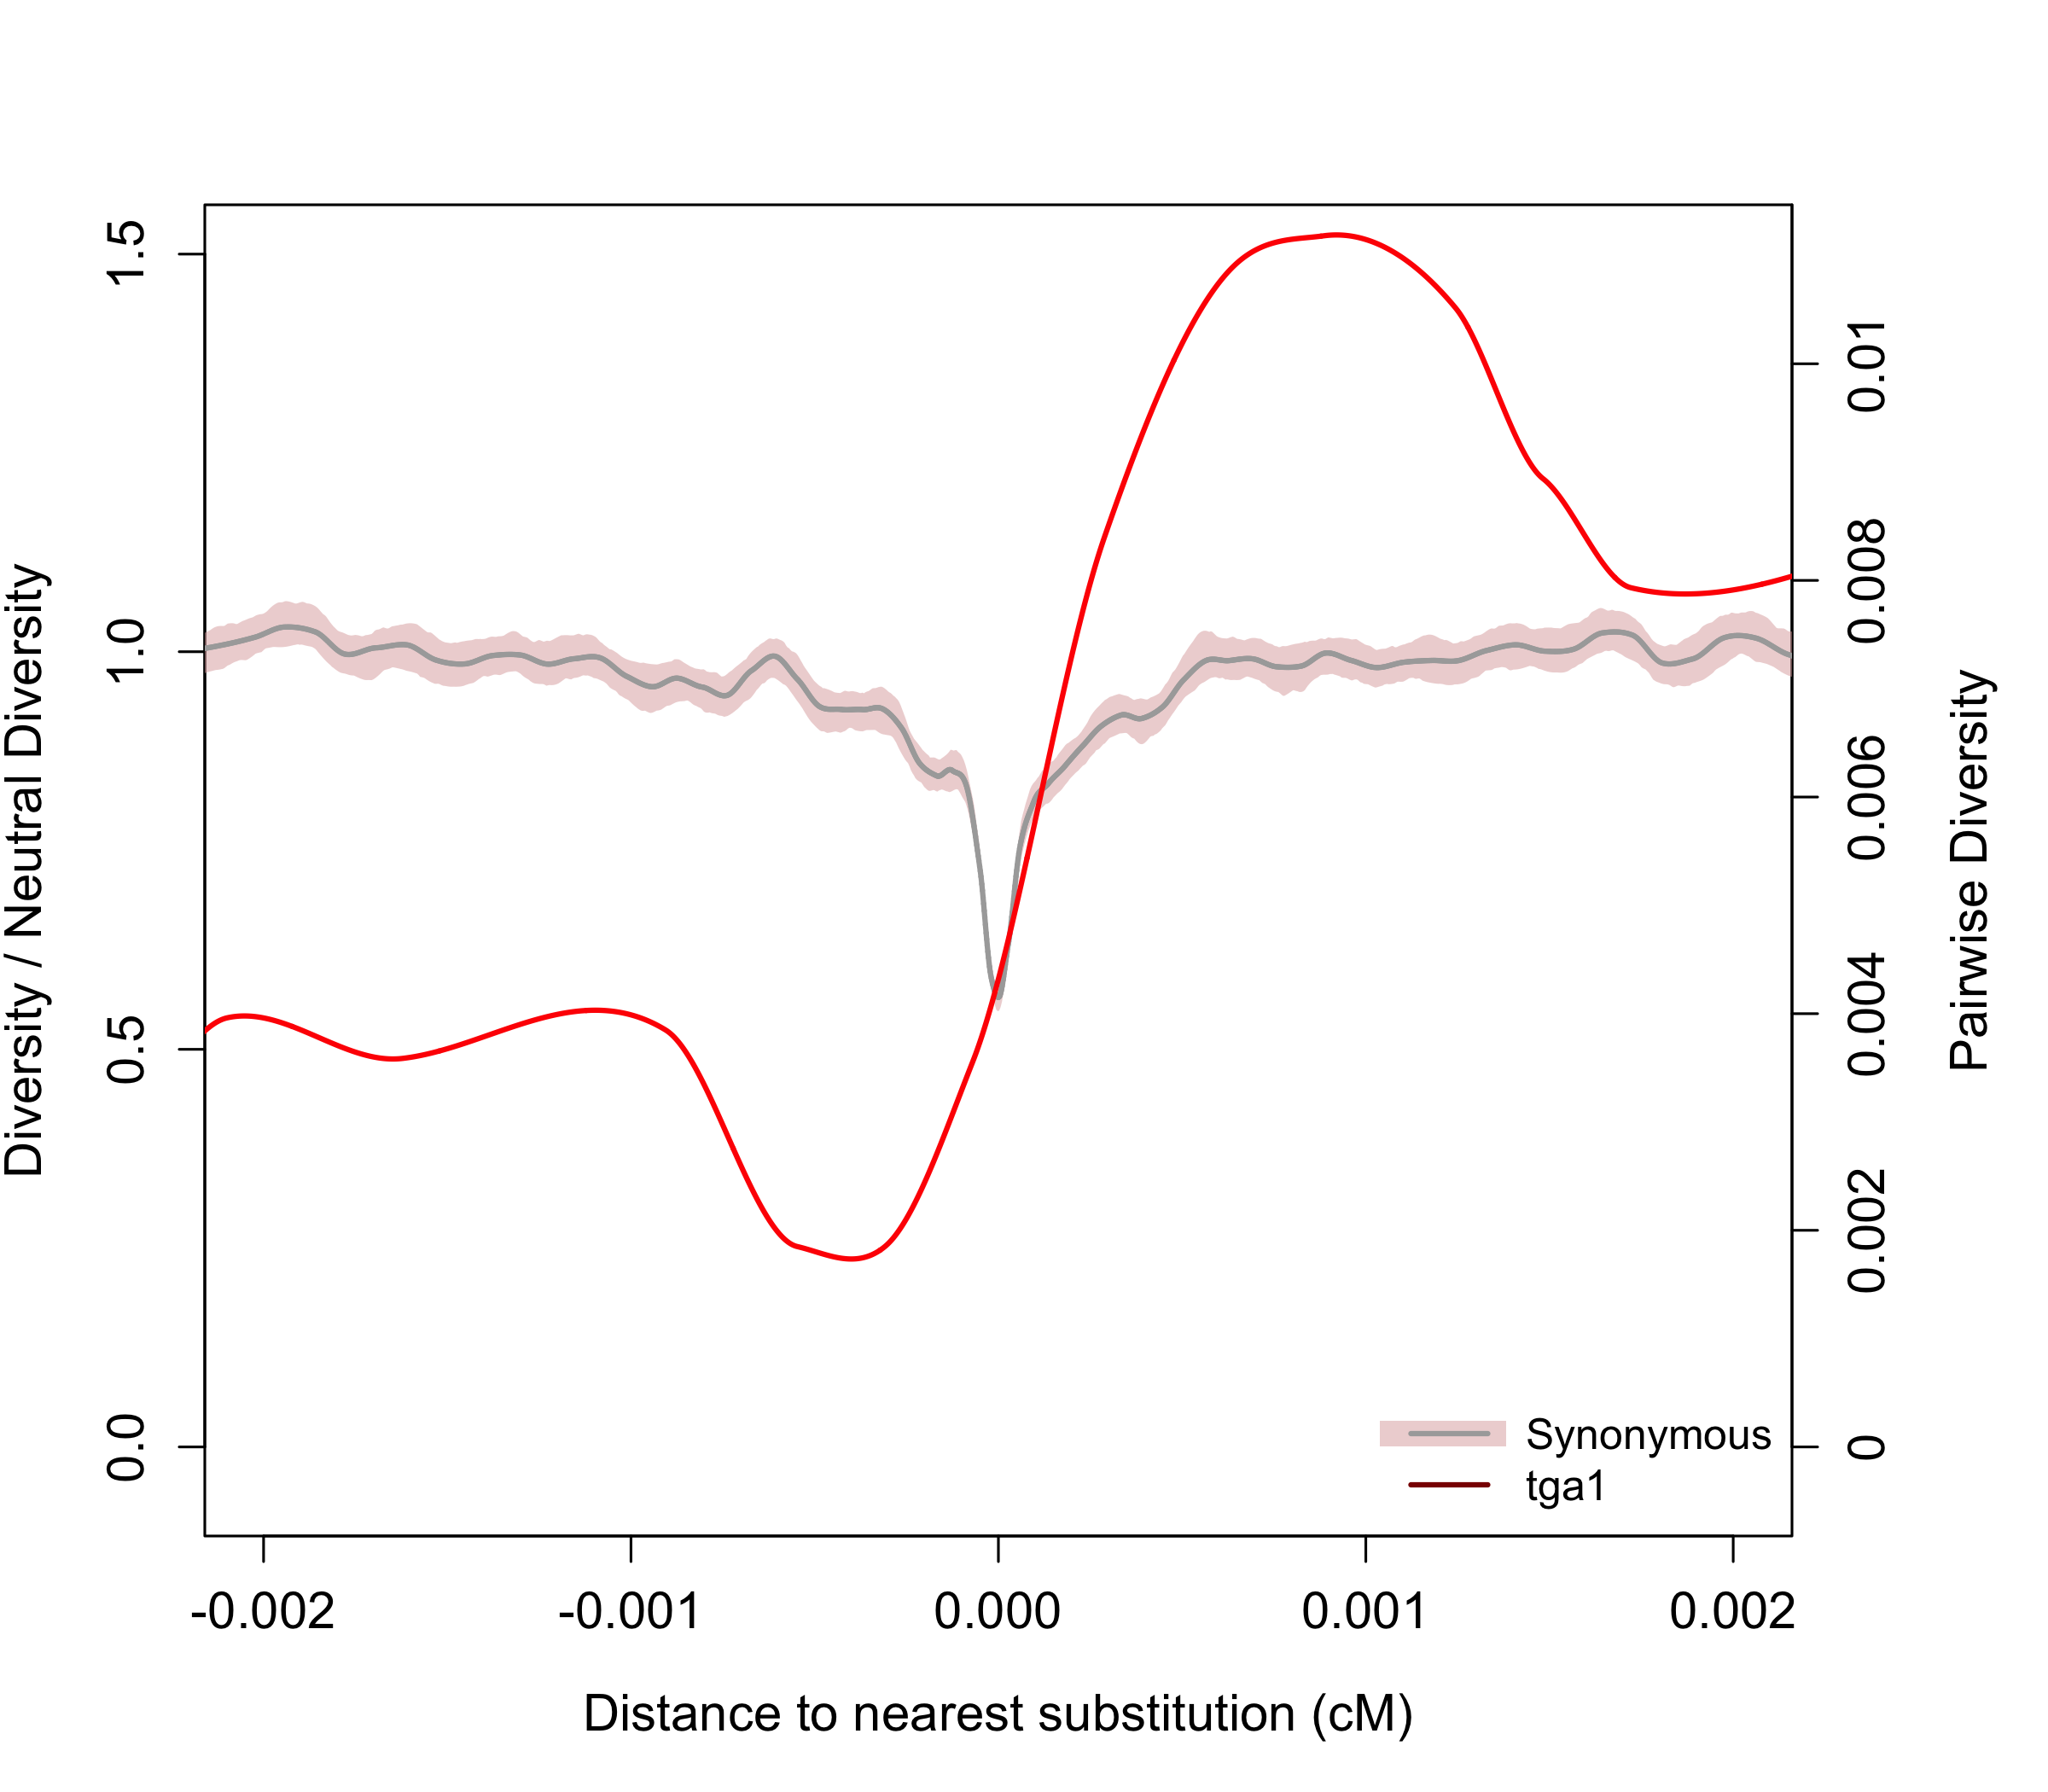
\includegraphics[width=\textwidth]{FigsAndFiles/plotDiversity_TvM_Folded2_Significance_tga1Supp_June.png}
    \end{center}
\caption{Diversity surrounding the causative substitution at the \emph{tga1} locus.  \label{sFig:tga1}}
\end{figure}
\clearpage

\begin{figure}
  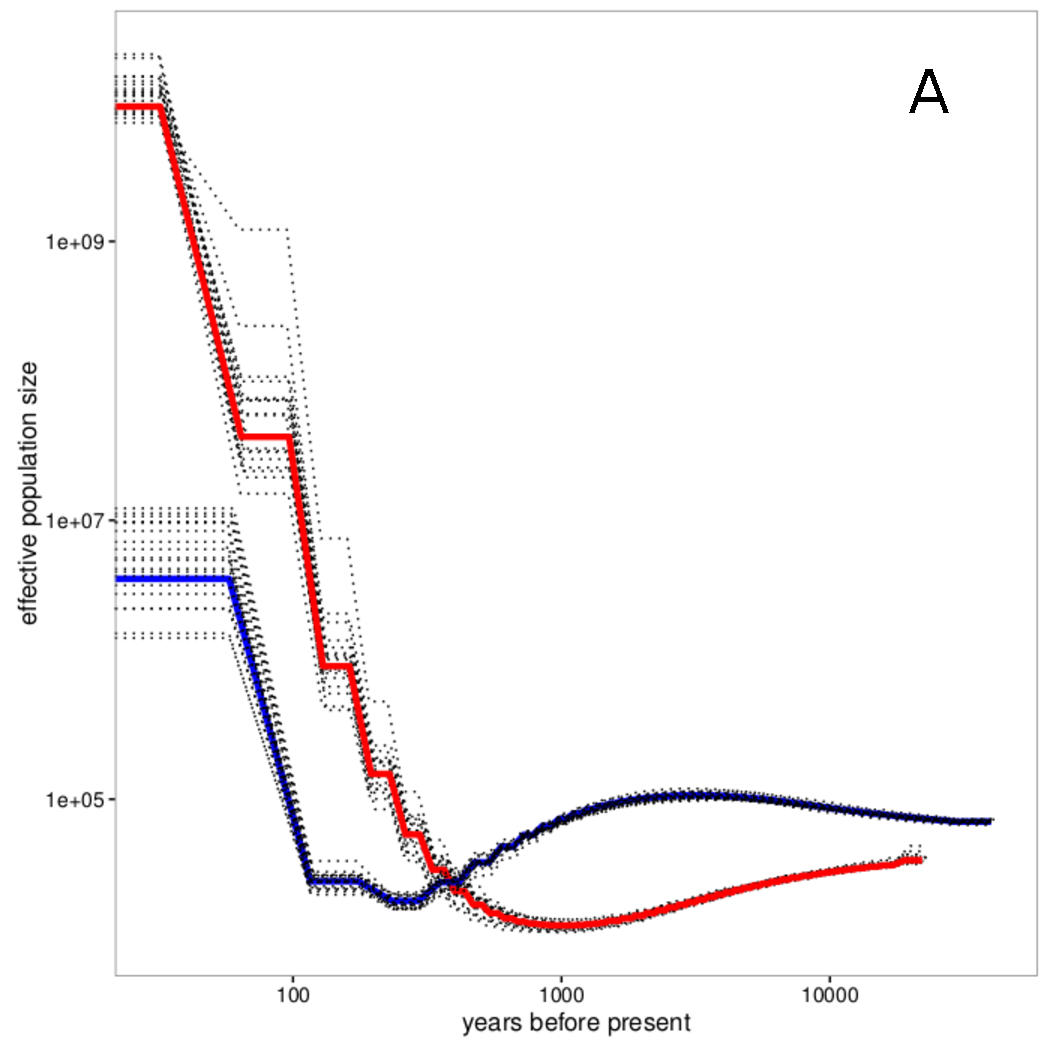
\includegraphics[width=.5\textwidth]{FigsAndFiles/TIL_BKN_bootstrapping_msmc2_labeled.pdf}
  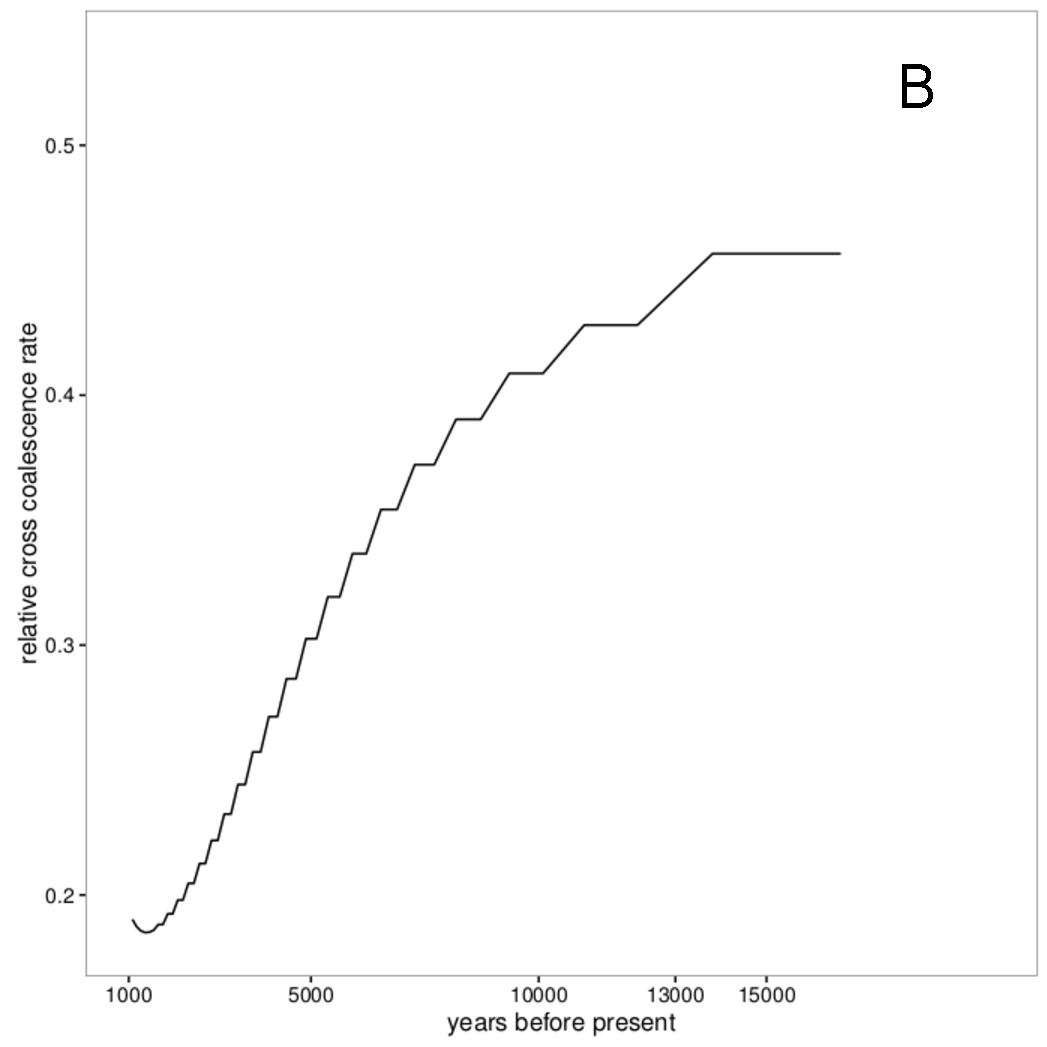
\includegraphics[width=.5\textwidth]{FigsAndFiles/relativeCrossCoalescenceRate_labeled.pdf}
\caption{MSMC Analyses. Shown in \textbf{A} are effective population size estimates over time. Estimates are depicted as solid lines and boostrap resampling is represented with dotted lines for both maize (red) and teosinte (blue). \textbf{B} depticts the cross-coalescence rate between maize and teosinte estimated using MSMC. In both panels, time is estimated assuming an annual generation time and a mutation rate of $\mu=3\times 10^{-8}$ \label{sFig:msmc}}
\end{figure}
\clearpage


\begin{figure}
  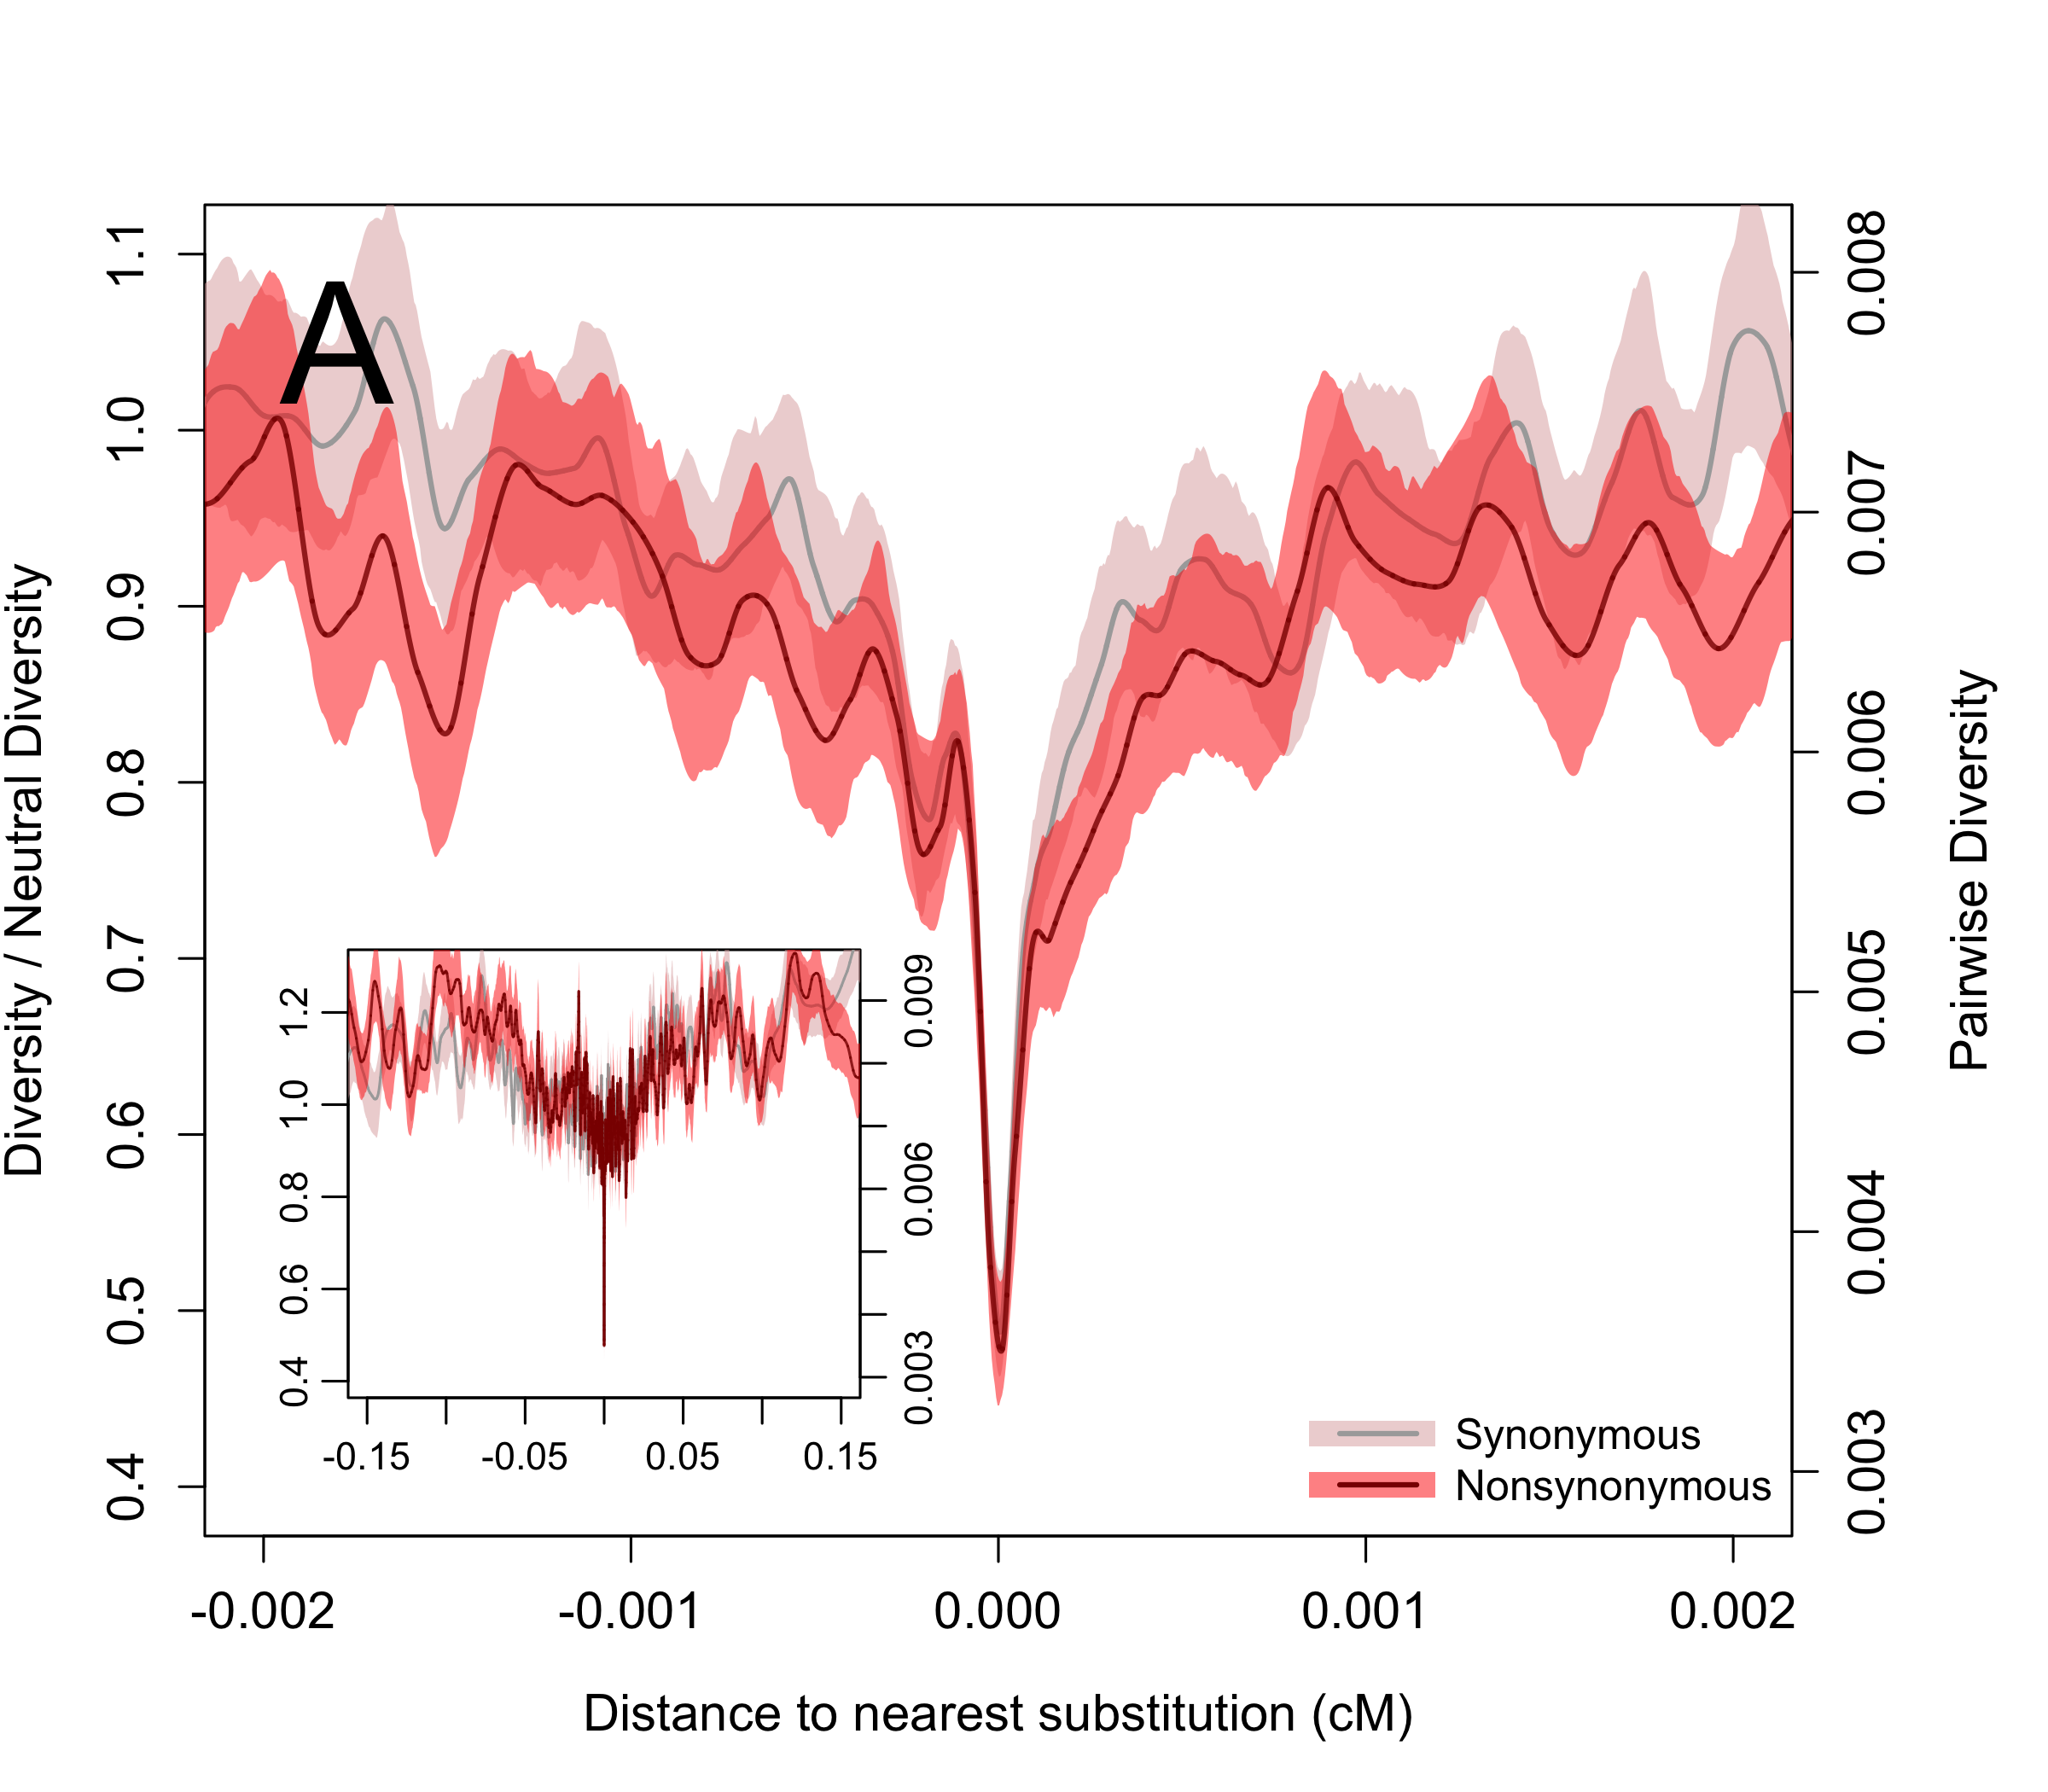
\includegraphics[width=.5\textwidth]{FigsAndFiles/plotDiversity_TvM_Conserved_Significance_June.png}
  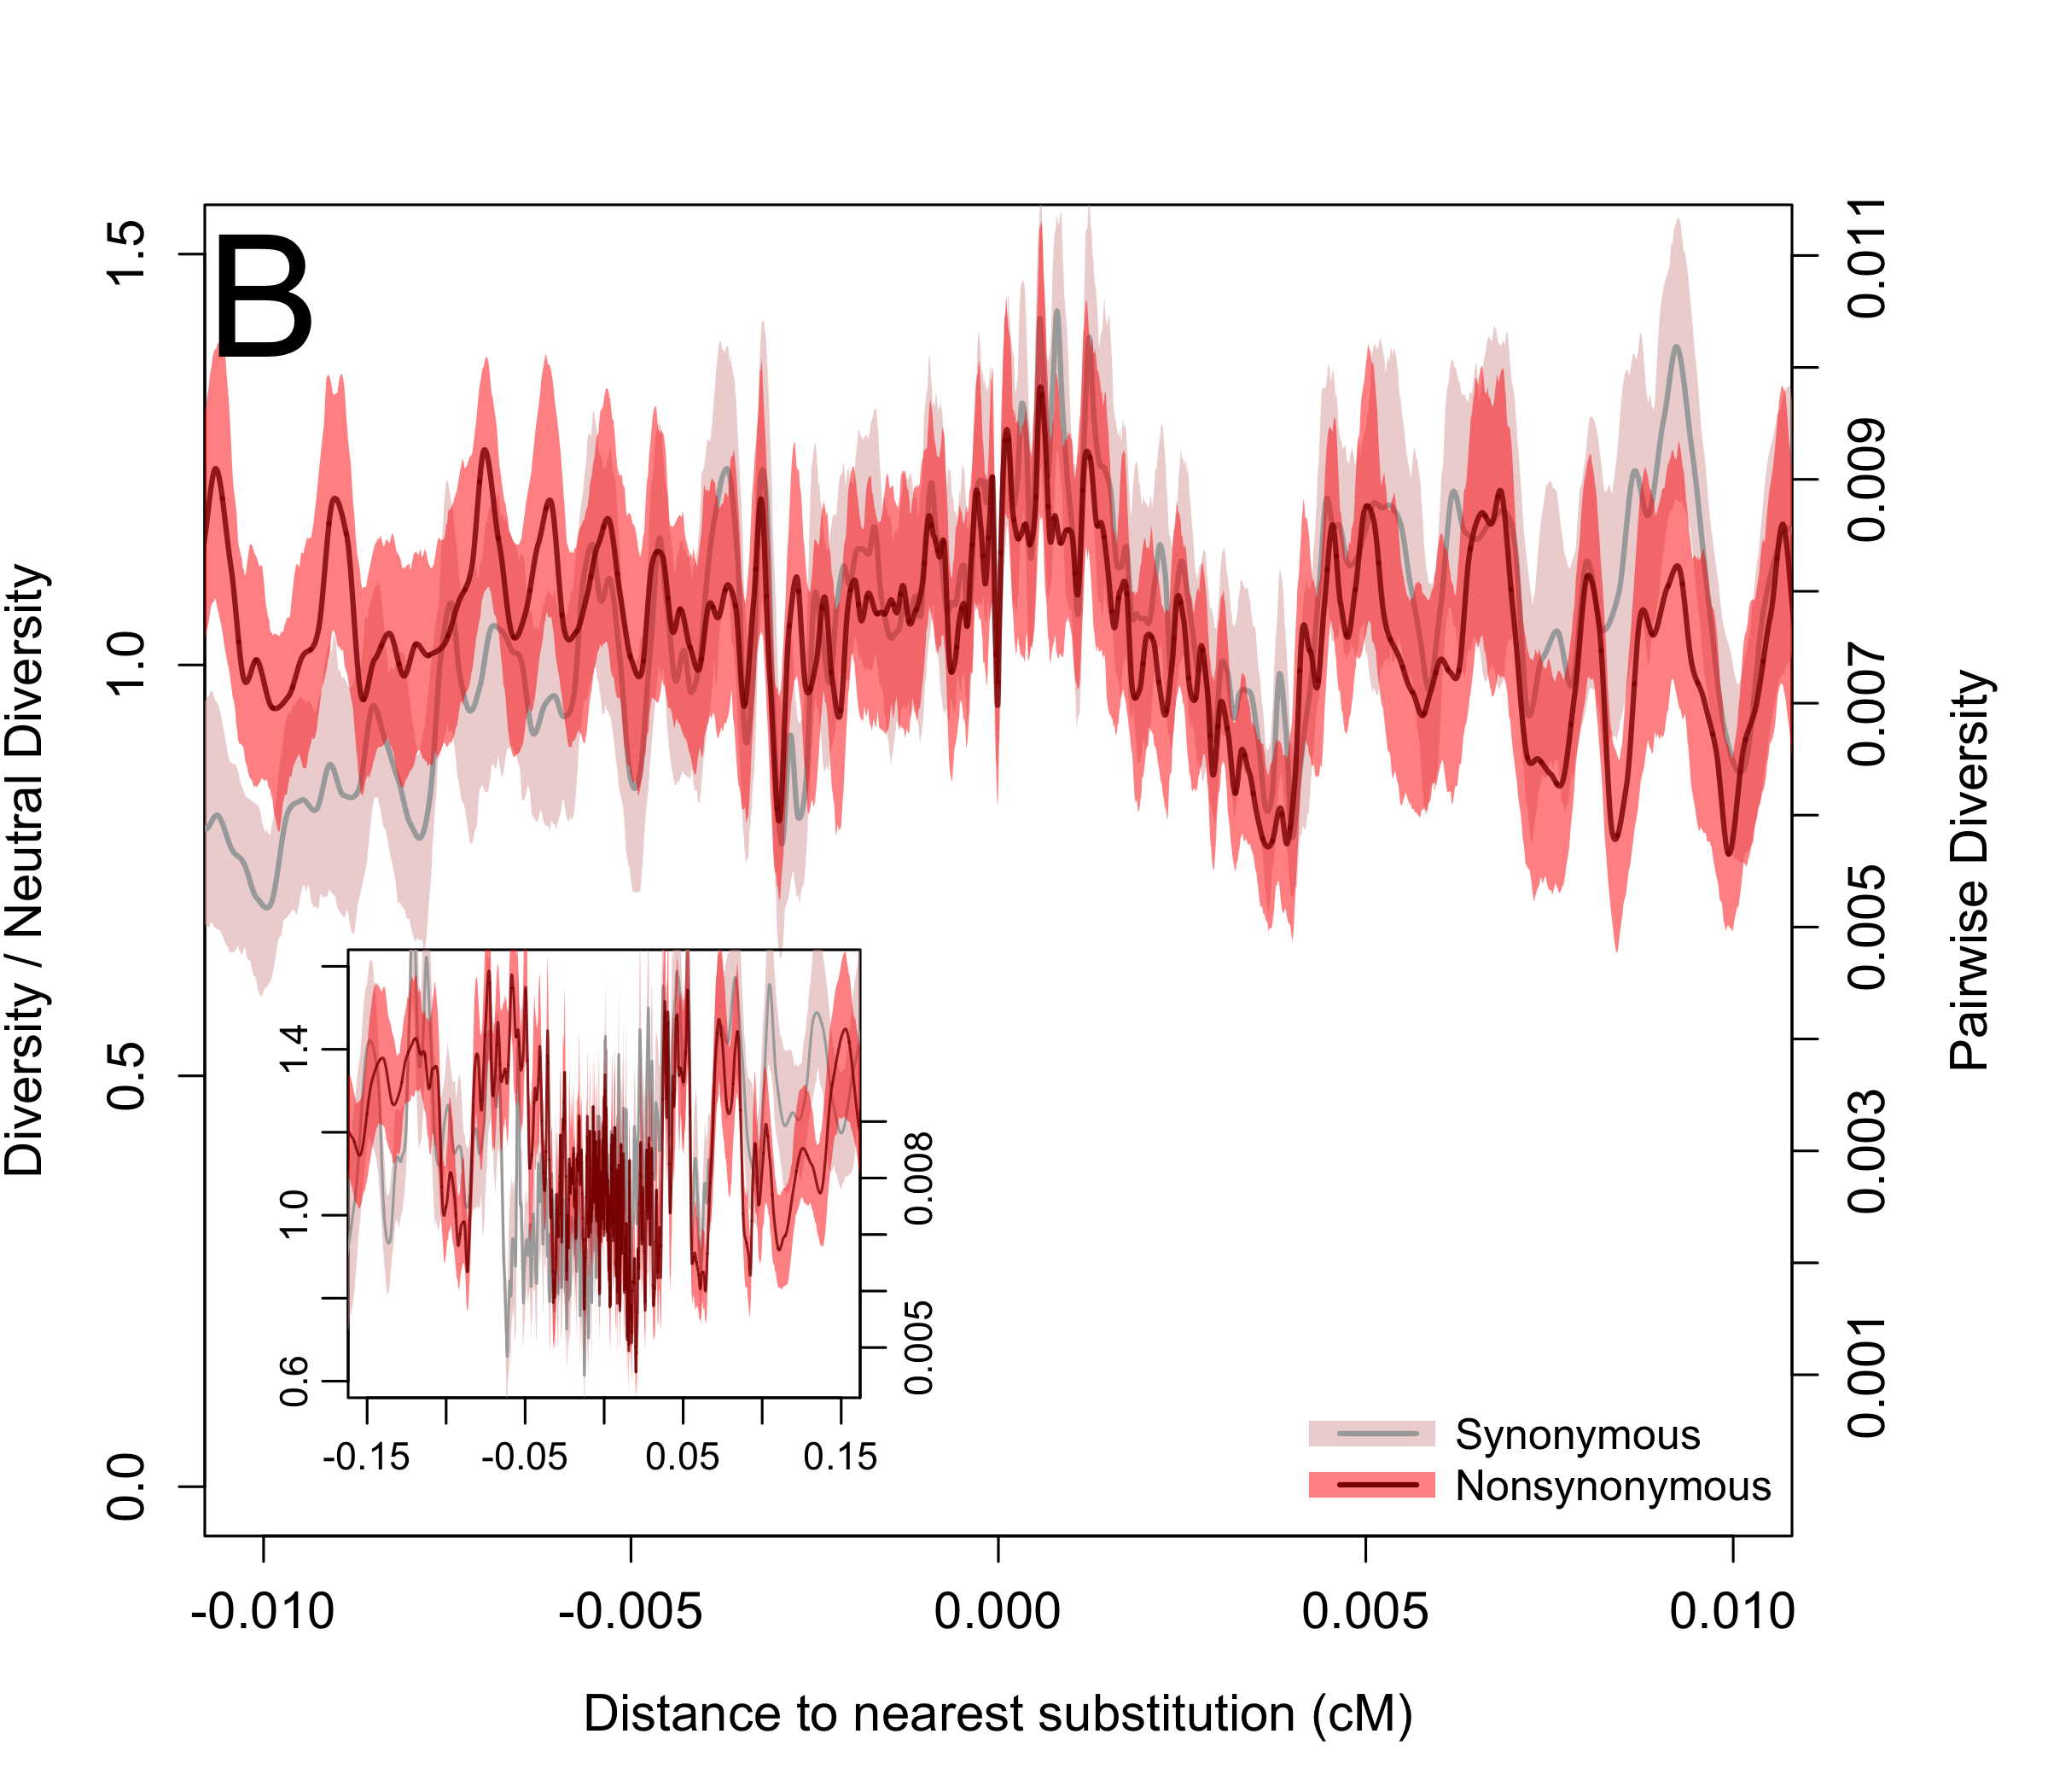
\includegraphics[width=.5\textwidth]{FigsAndFiles/plotDiversity_TvM_Unconserved_Significance_June.png}
\caption{ Pairwise diversity surrounding synonymous and nonsynonymous
  substitutions in maize at \textbf{A} highly conserved or \textbf{B}  unconserved sites.  Bootstrap-based 95\% confidence intervals are depicted via shading. Inset plots depict a larger range on the x-axis. \label{sFig:consUncons}}
\end{figure}
\clearpage

\begin{figure}
  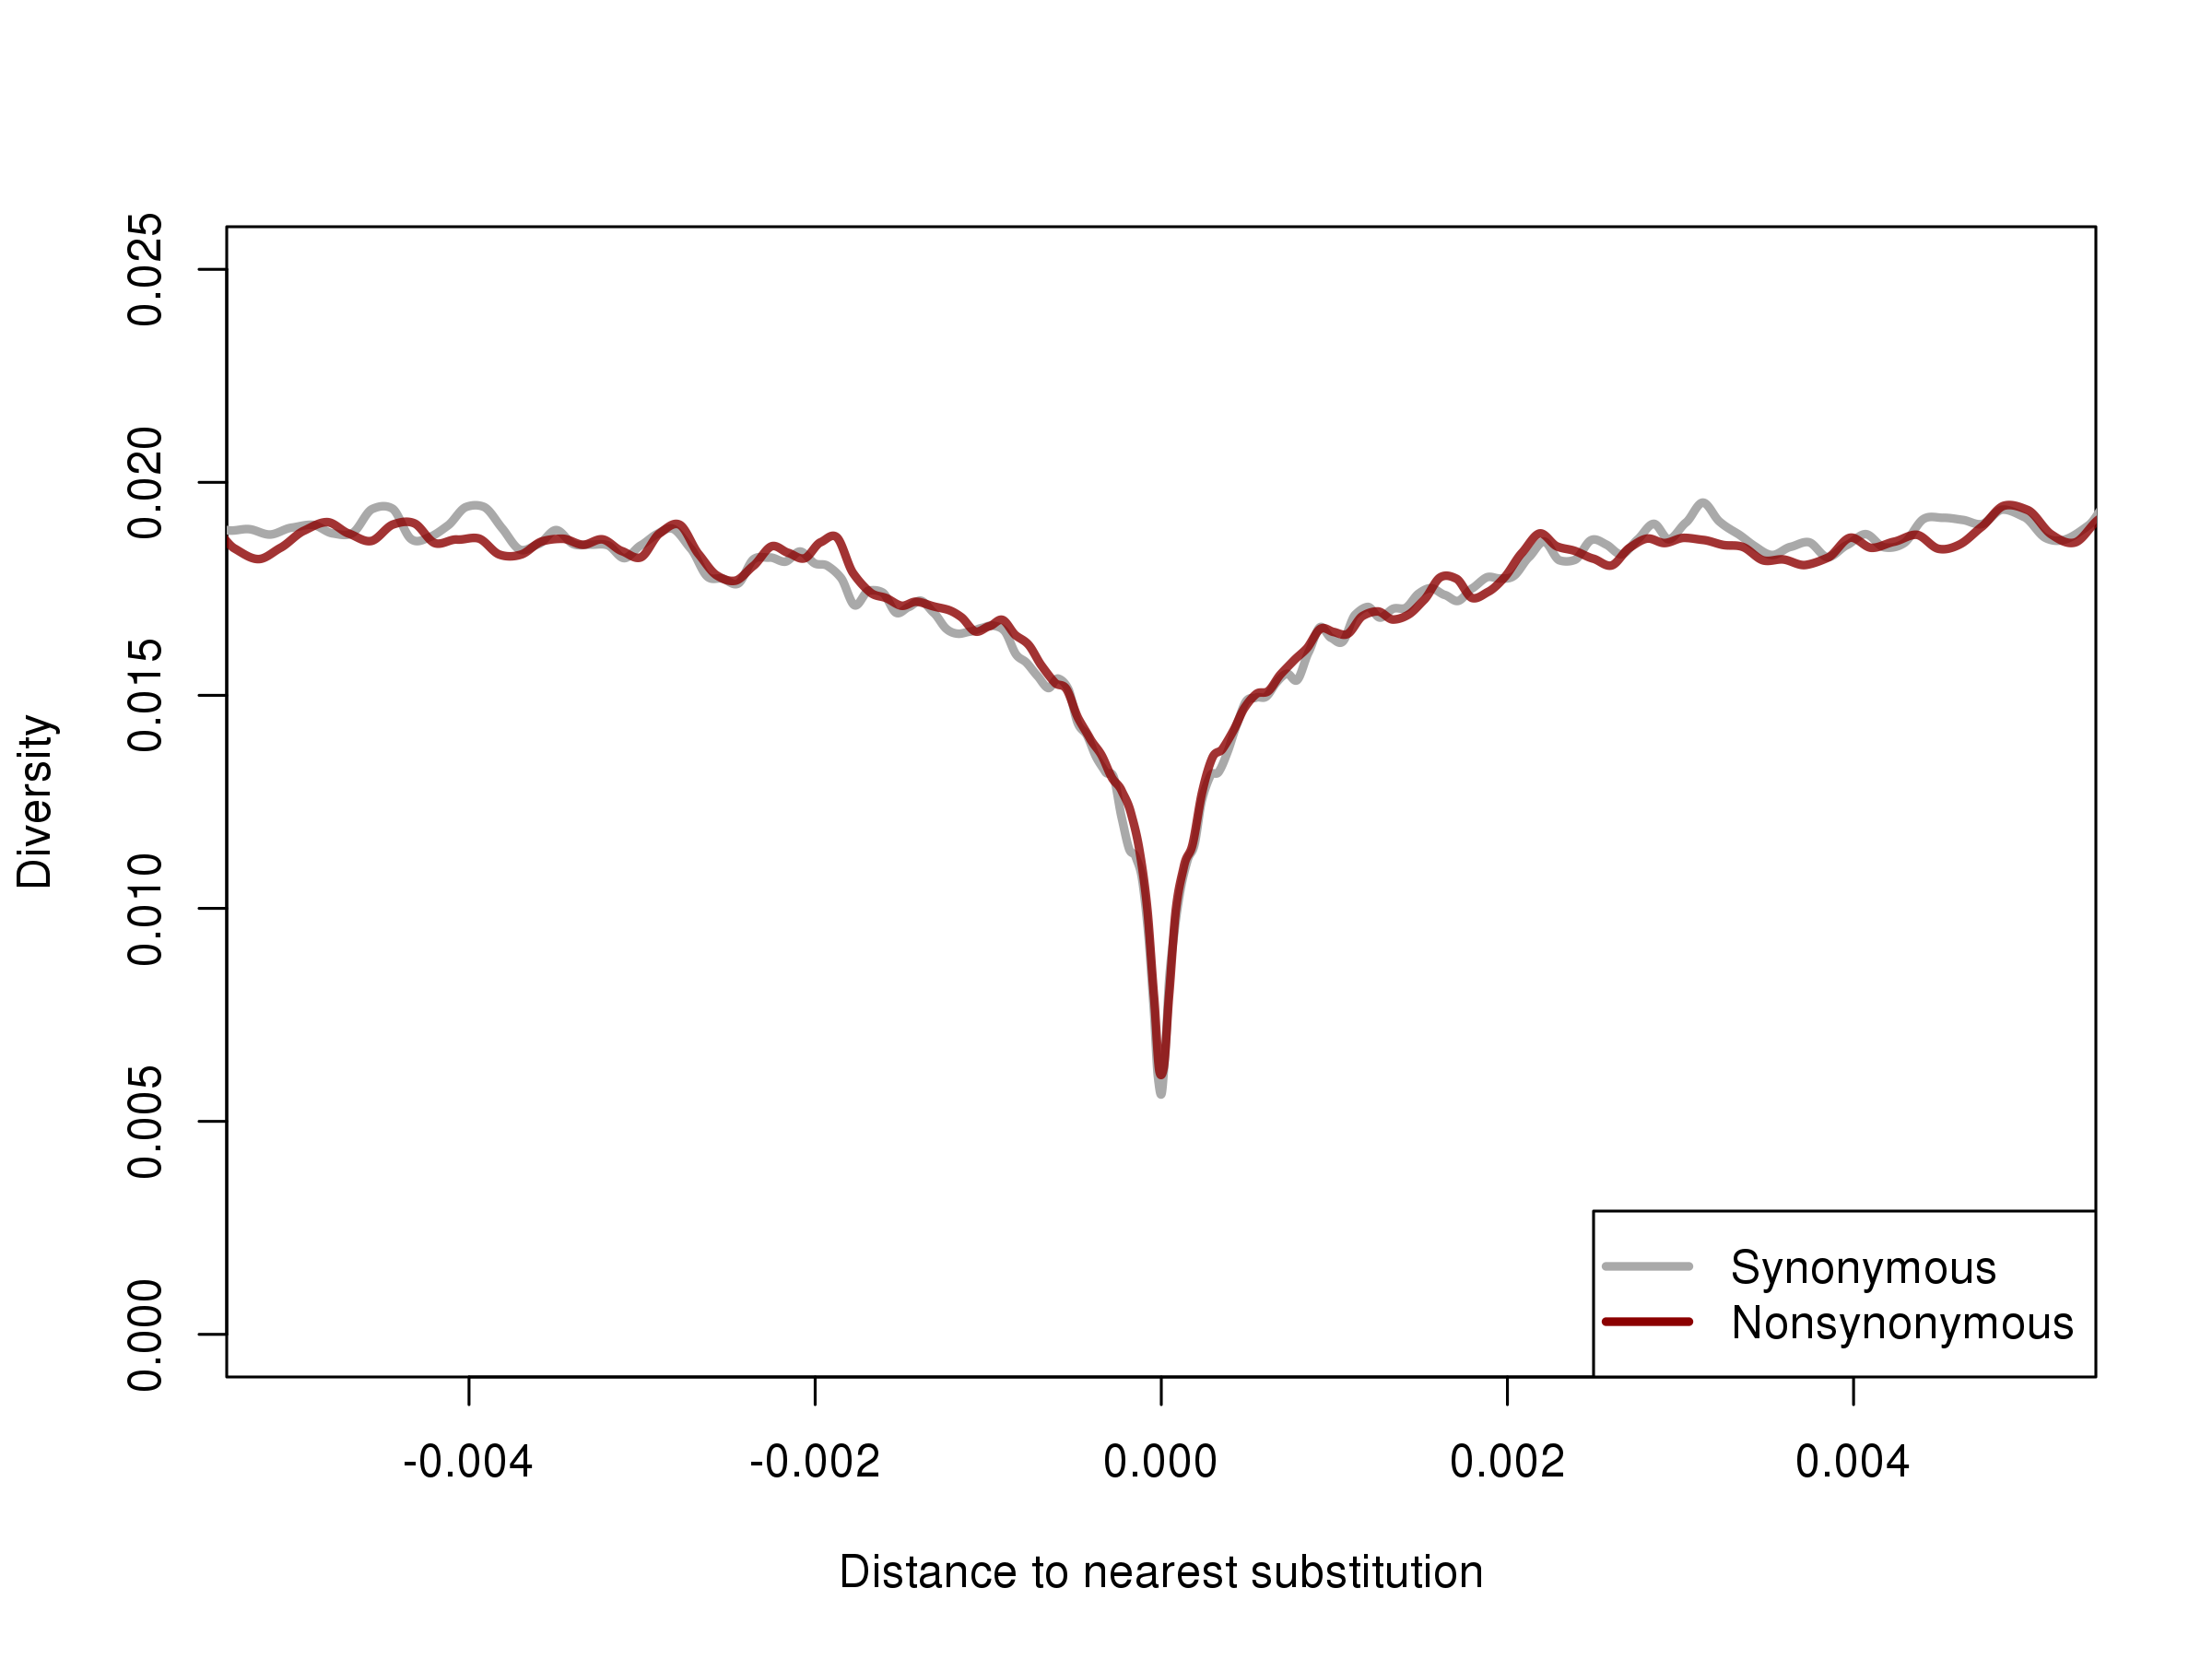
\includegraphics[width=\textwidth]{FigsAndFiles/plotDiversity_TvM_Singletons.png}
\caption{ Singleton diversity surrounding synonymous and nonsynonymous
  substitutions in maize. \label{sFig:singleton}}
\end{figure}
\clearpage

\begin{figure}
  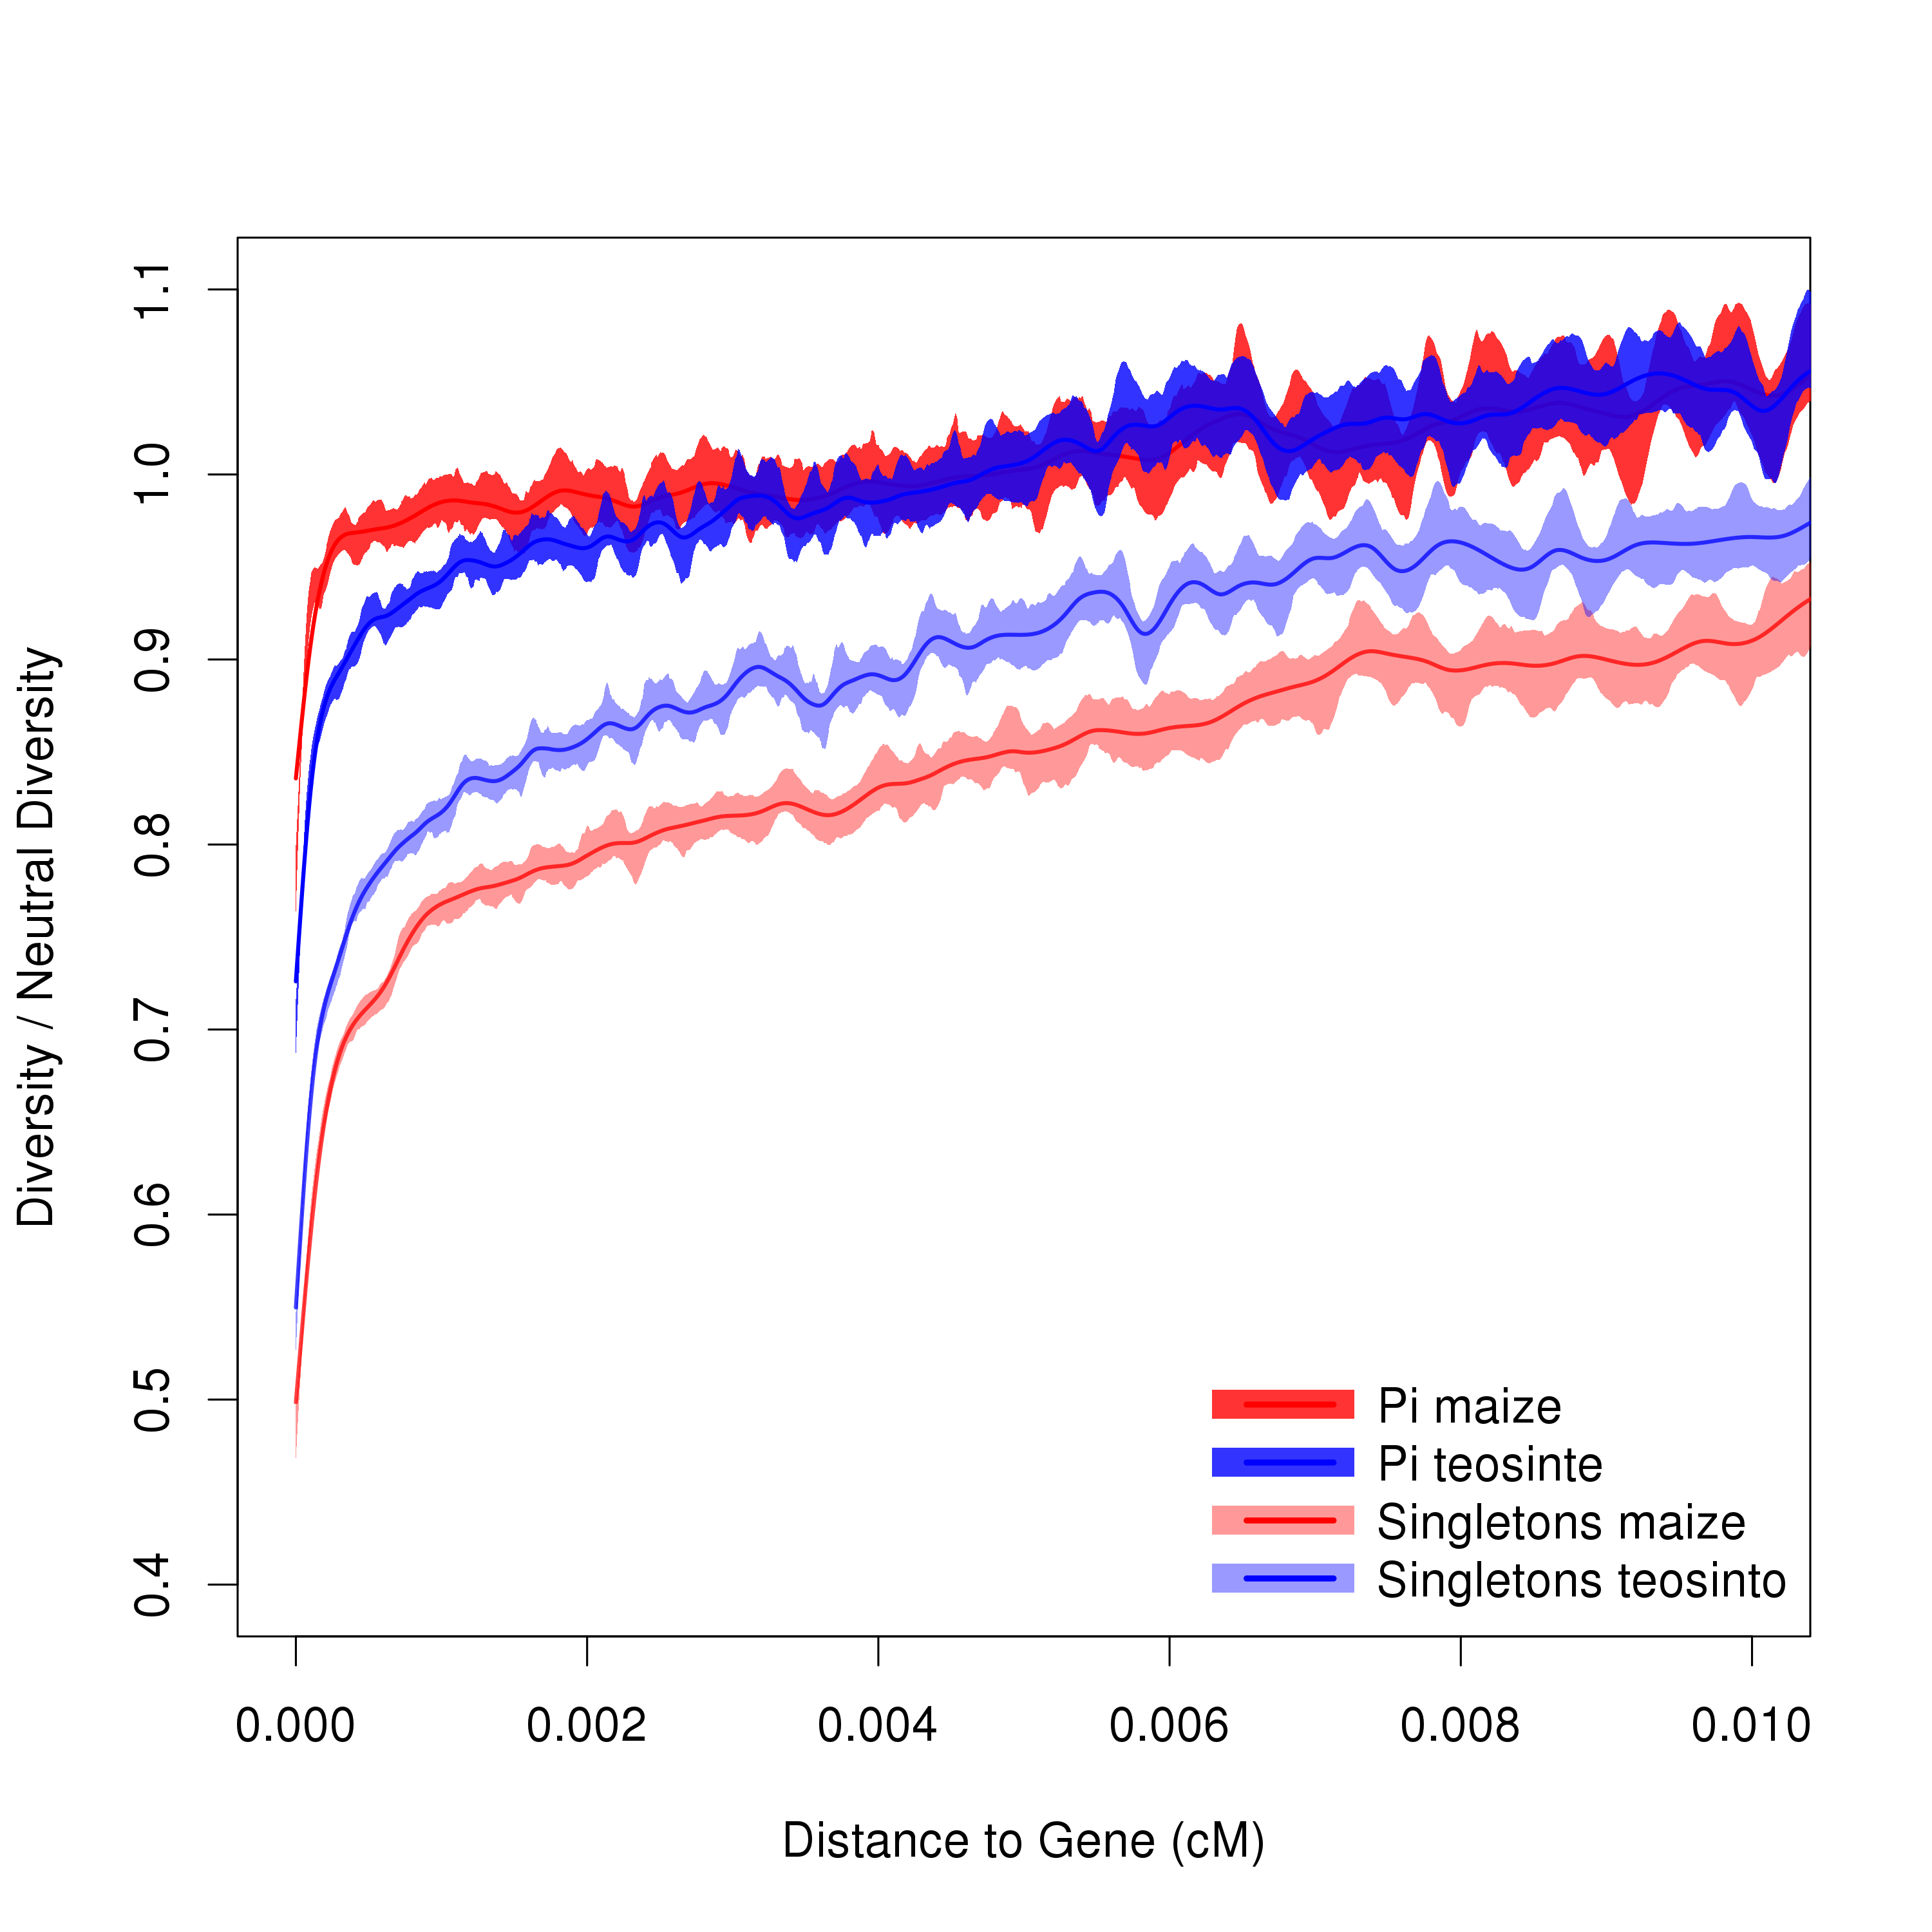
\includegraphics[width=\textwidth]{FigsAndFiles/distanceToGene_WithSignificance_Folded2_maizeAndTeoSingleVsPi.png}
\caption{ Relative diversity versus distance to nearest gene in maize and teosinte. Relative diversity is calculated by comparing to the mean diversity in all windows $\geq 0.02 cM$ from the nearest gene. Lines depict cubic smoothing splines with smoothing parameters chosen via generalized cross validation and shading depicts bootstrap-based 95\% confidence intervals.  \label{sFig:singletonPi}}
\end{figure}
\clearpage

\begin{figure}
  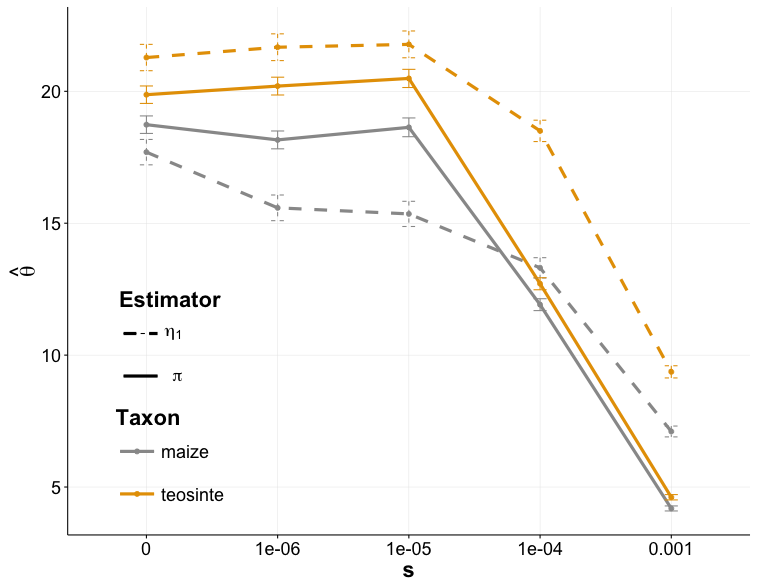
\includegraphics[width=\textwidth]{FigsAndFiles/jri_sims.png}
\caption{Simulations of diversity statistics in maize and teosinte with varying strengths of purifying selection. Points show the mean ($\pm$ standard error) of the population mutation rate $\theta$ estimated by singletons ($\eta_1$) and pairwise differences ($\pi$). \label{sFig:sims}}
\end{figure}
\clearpage


\begin{figure}
  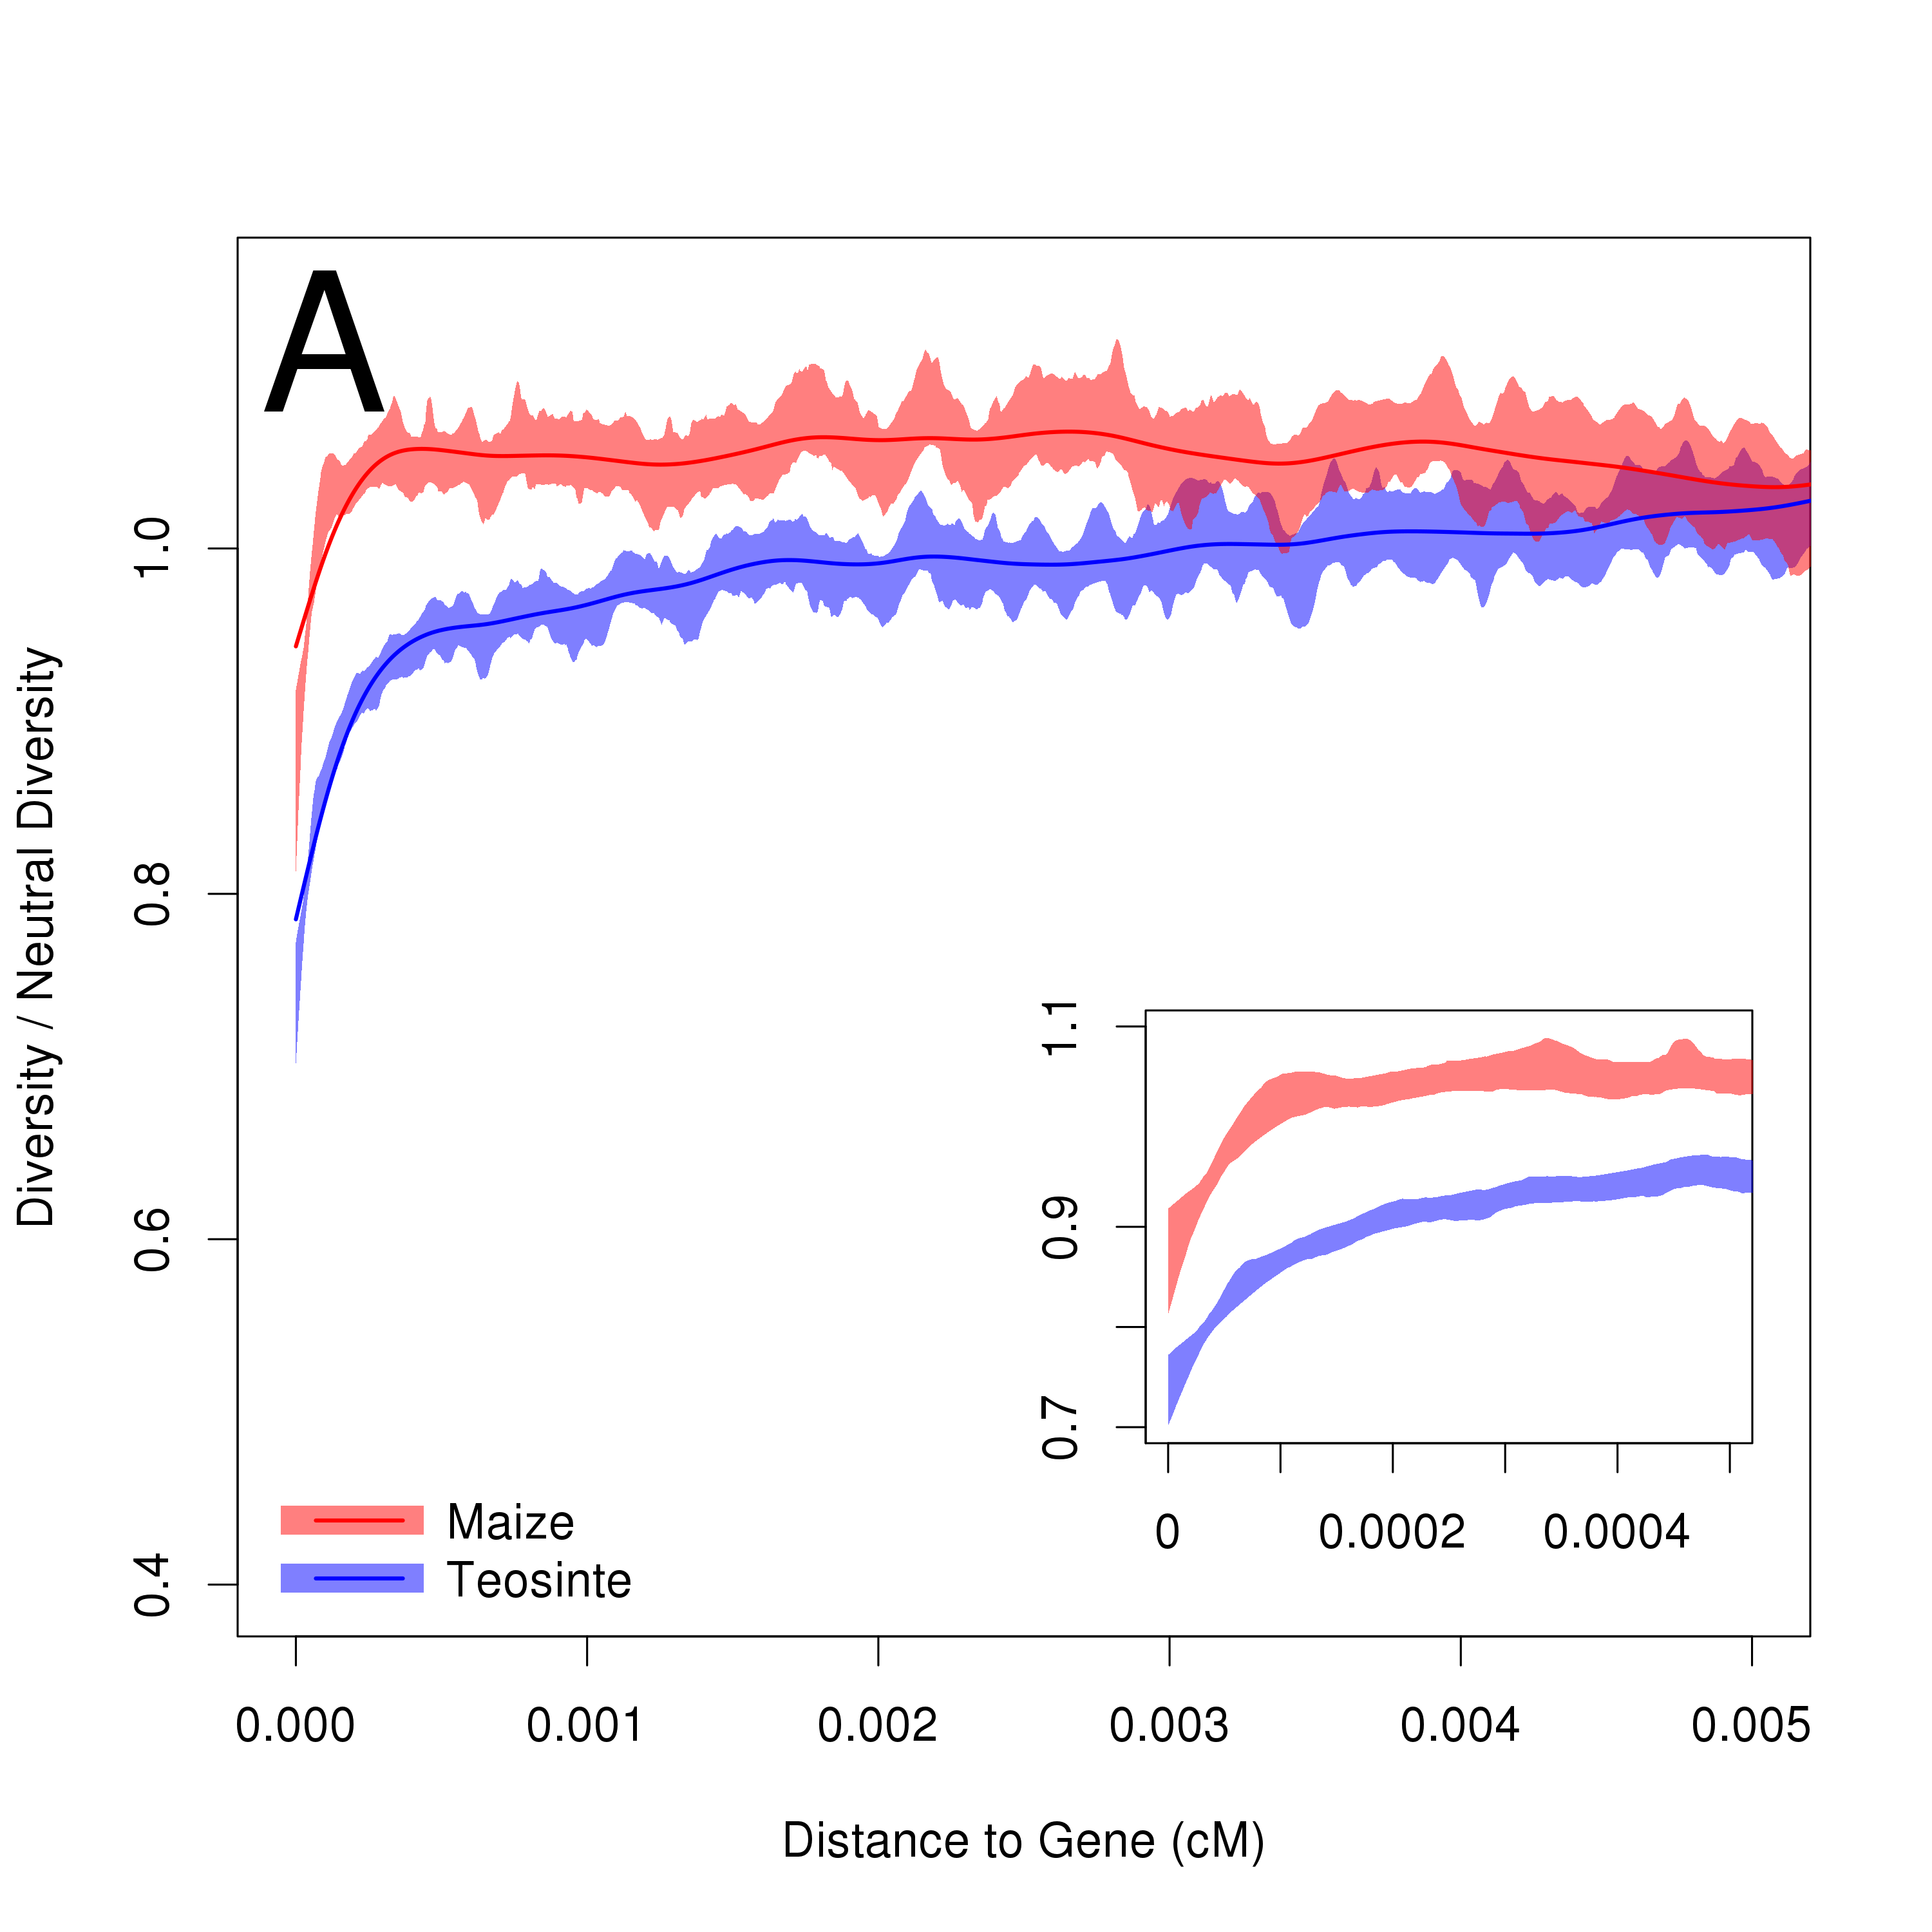
\includegraphics[width=.5\textwidth]{FigsAndFiles/distanceToGene_Unselected_manuscript.png}
    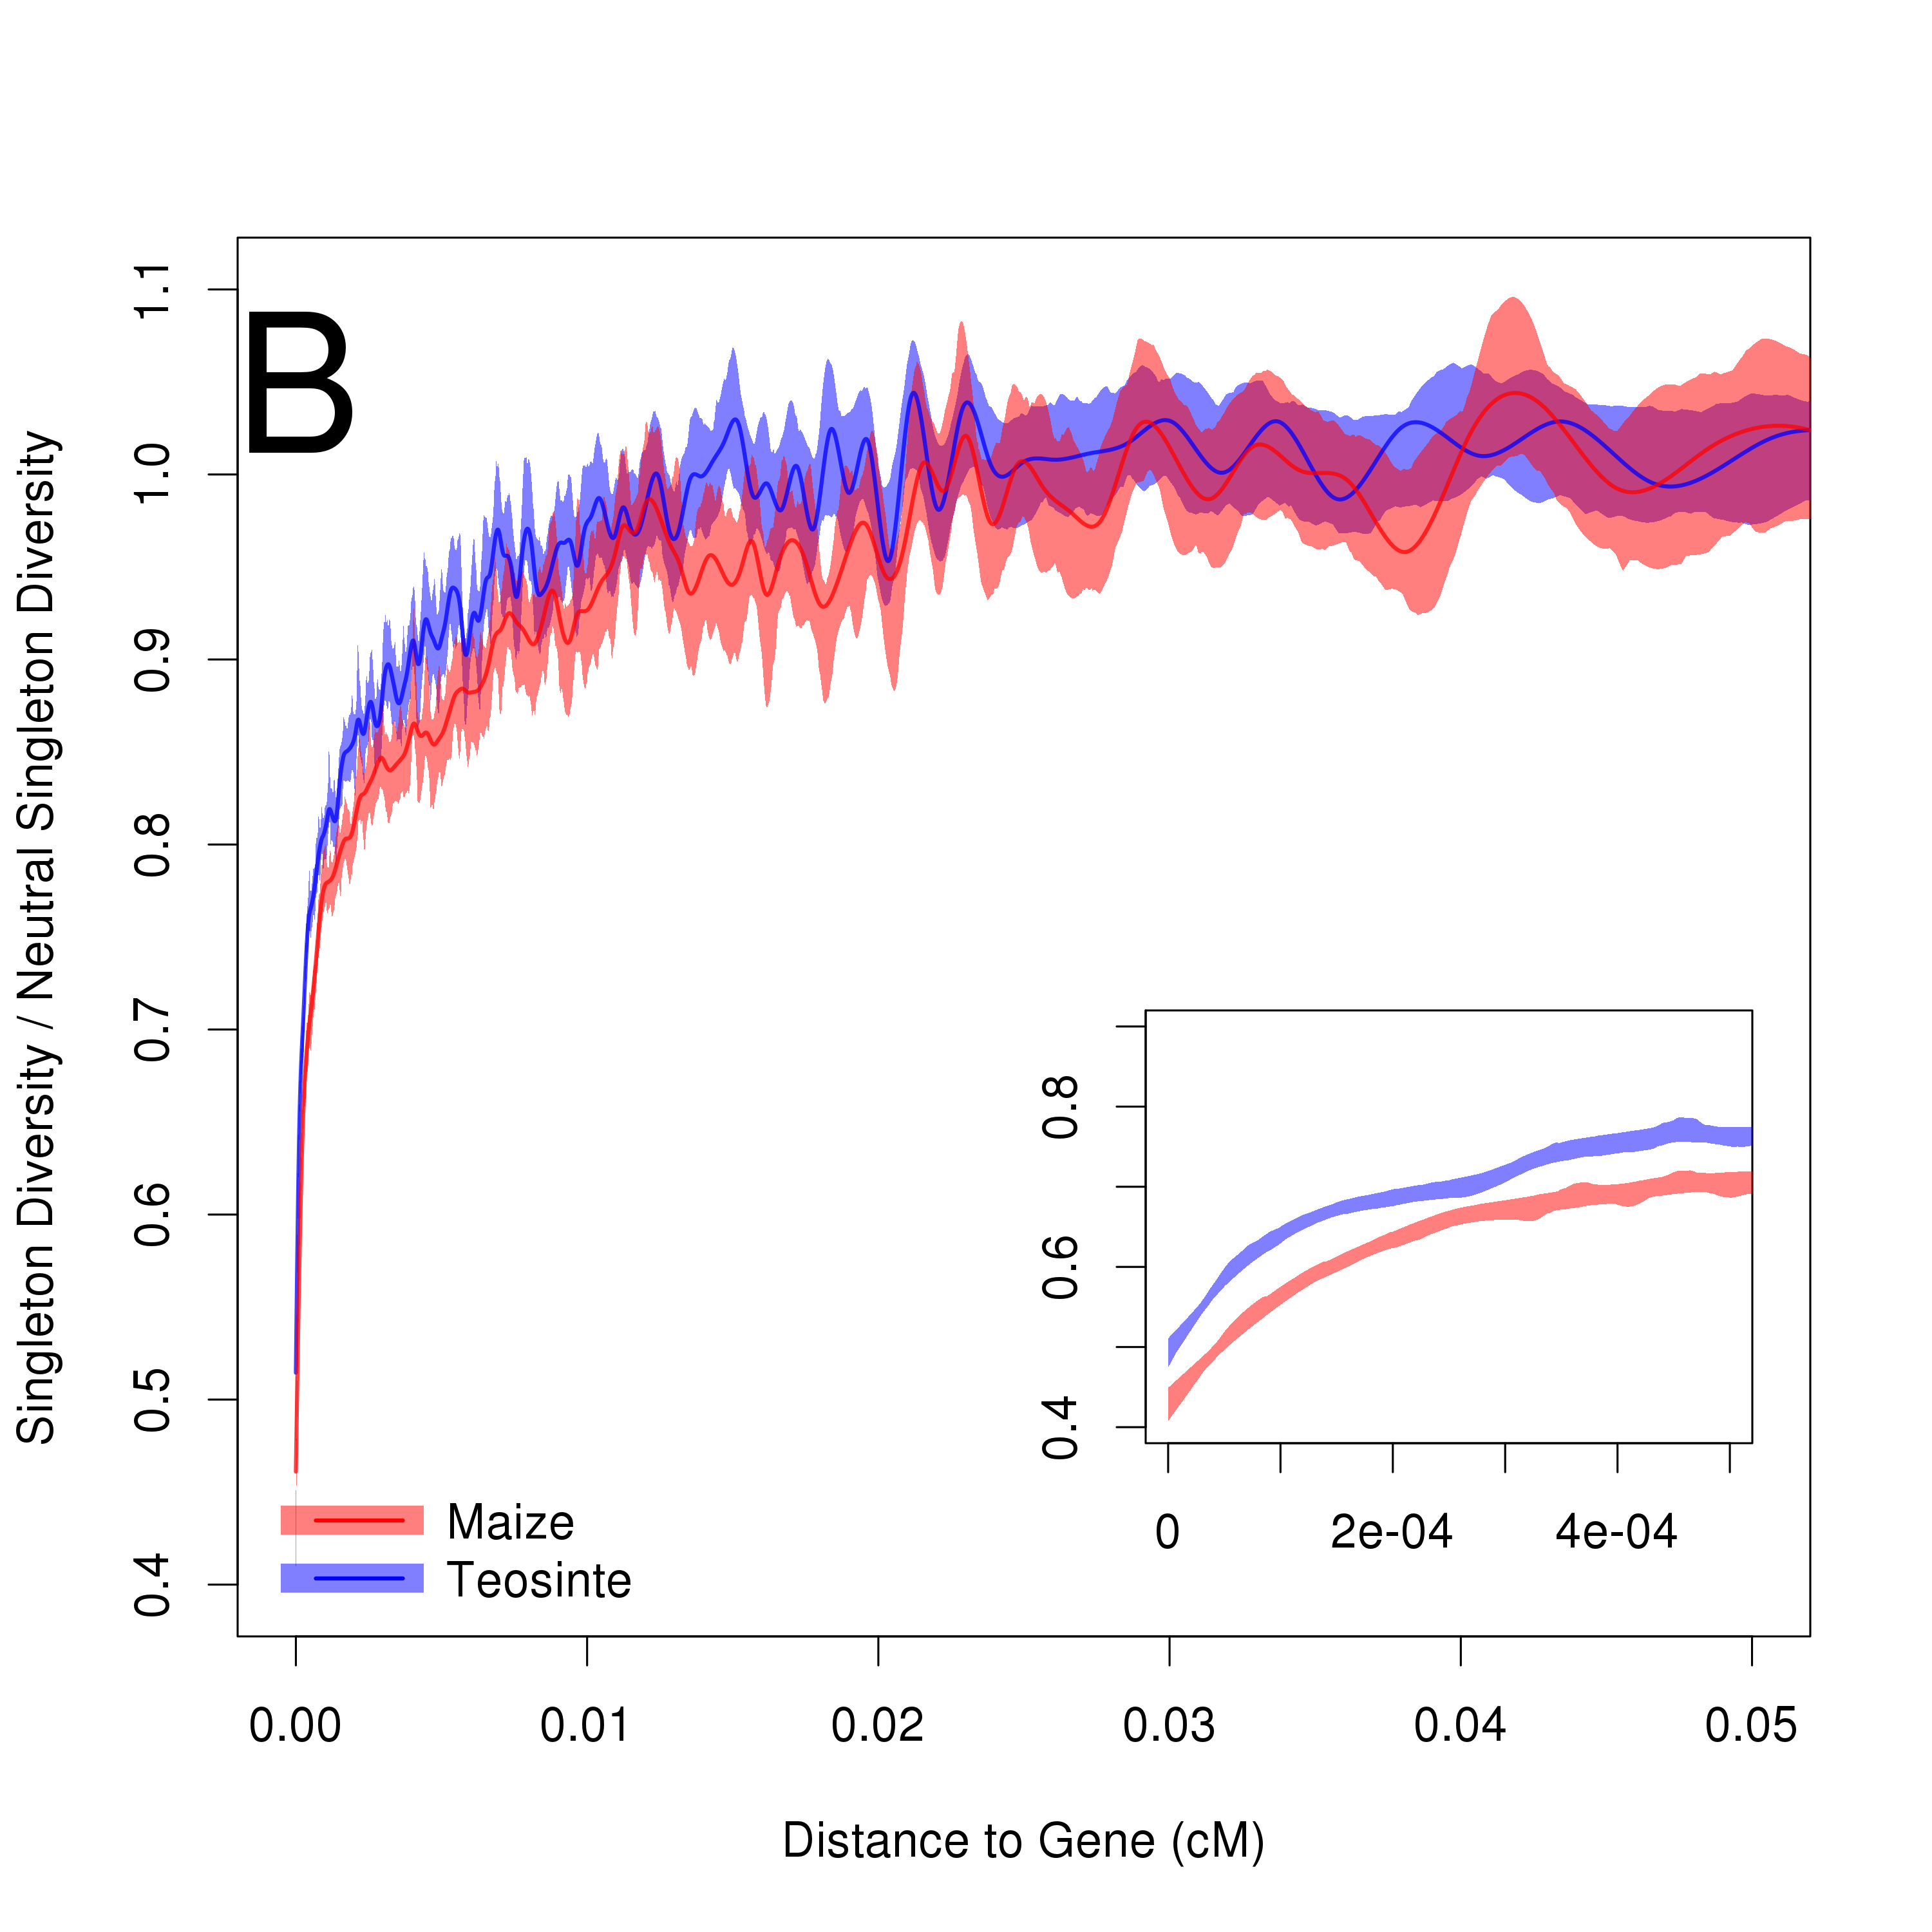
\includegraphics[width=.5\textwidth]{FigsAndFiles/distanceToGene_unselected_Singletons_manuscript.png}
\caption{ Relative level of diversity versus distance to the nearest gene, in maize and teosinte, based on only sites that do not show evidence of hard or soft sweeps according to H12. Two measures of diversity were investigated. {\bf A} displays pairwise diversity,
which is most influenced by intermediate frequency alleles and therefore depicts more ancient evolutionary patterns, and {\bf B} depicts singleton diversity, influenced by rare alleles and thus depicting evolutionary patterns in the recent past. Bootstrap-based 95\% confidence intervals are depicted via shading. Inset plots depict a smaller range on the x-axis. \label{sFig:H12}}
\end{figure}
\clearpage


\begin{figure}
  \begin{center}
  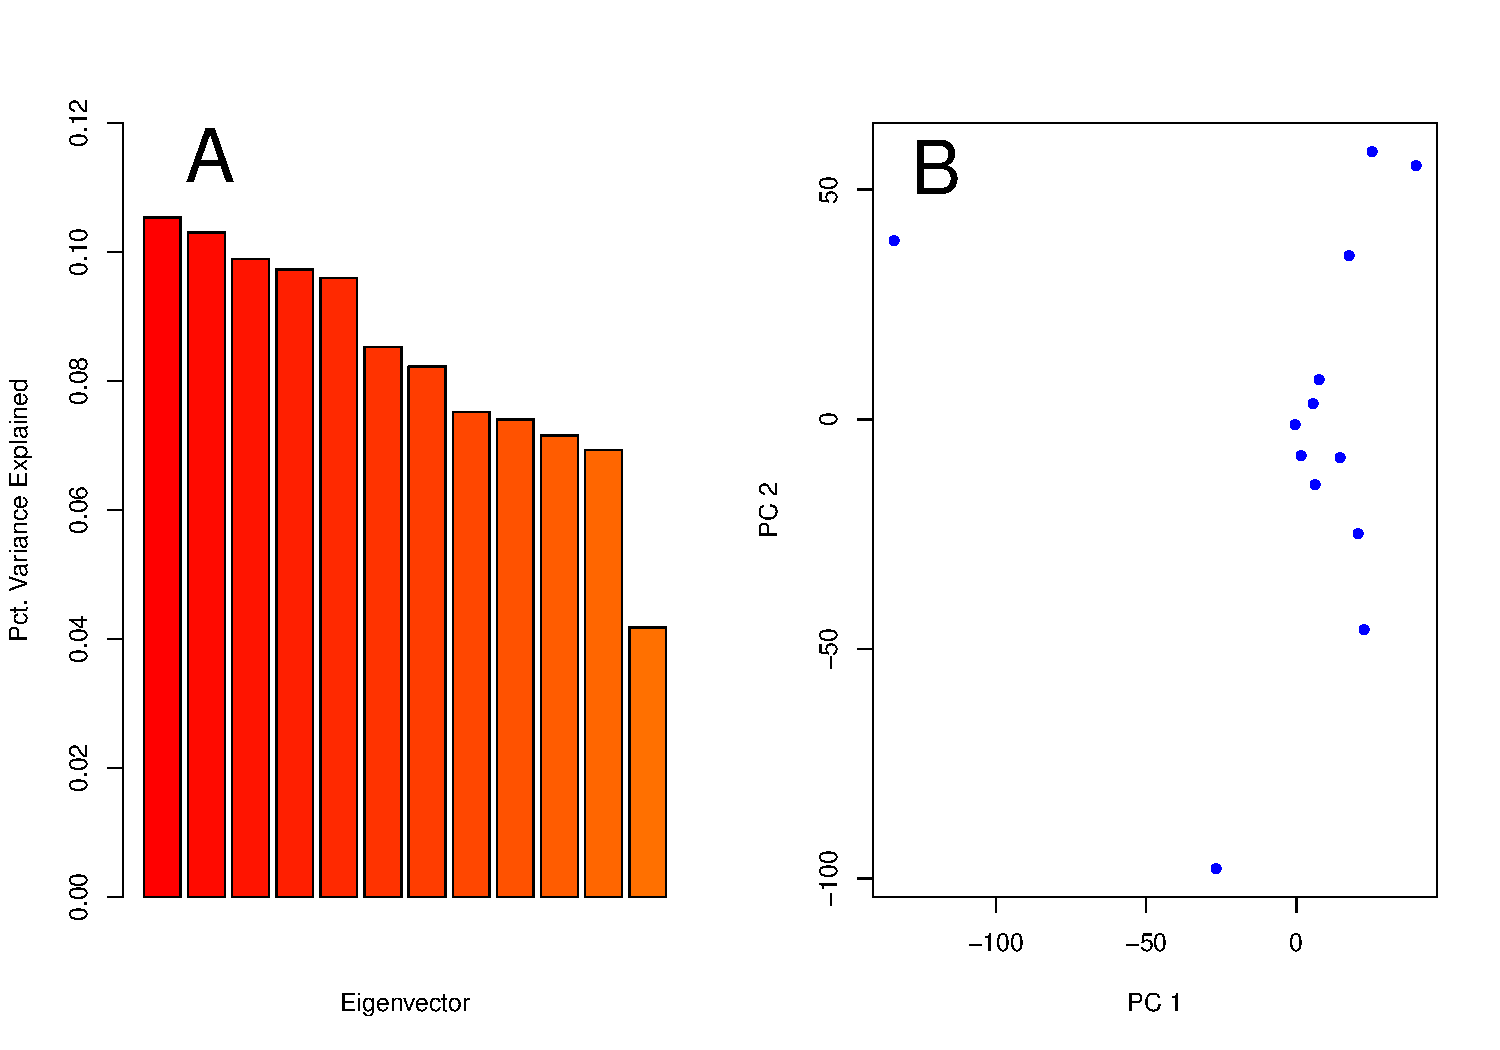
\includegraphics[width=.75\textwidth]{FigsAndFiles/tilPCA_aug.pdf}\\
  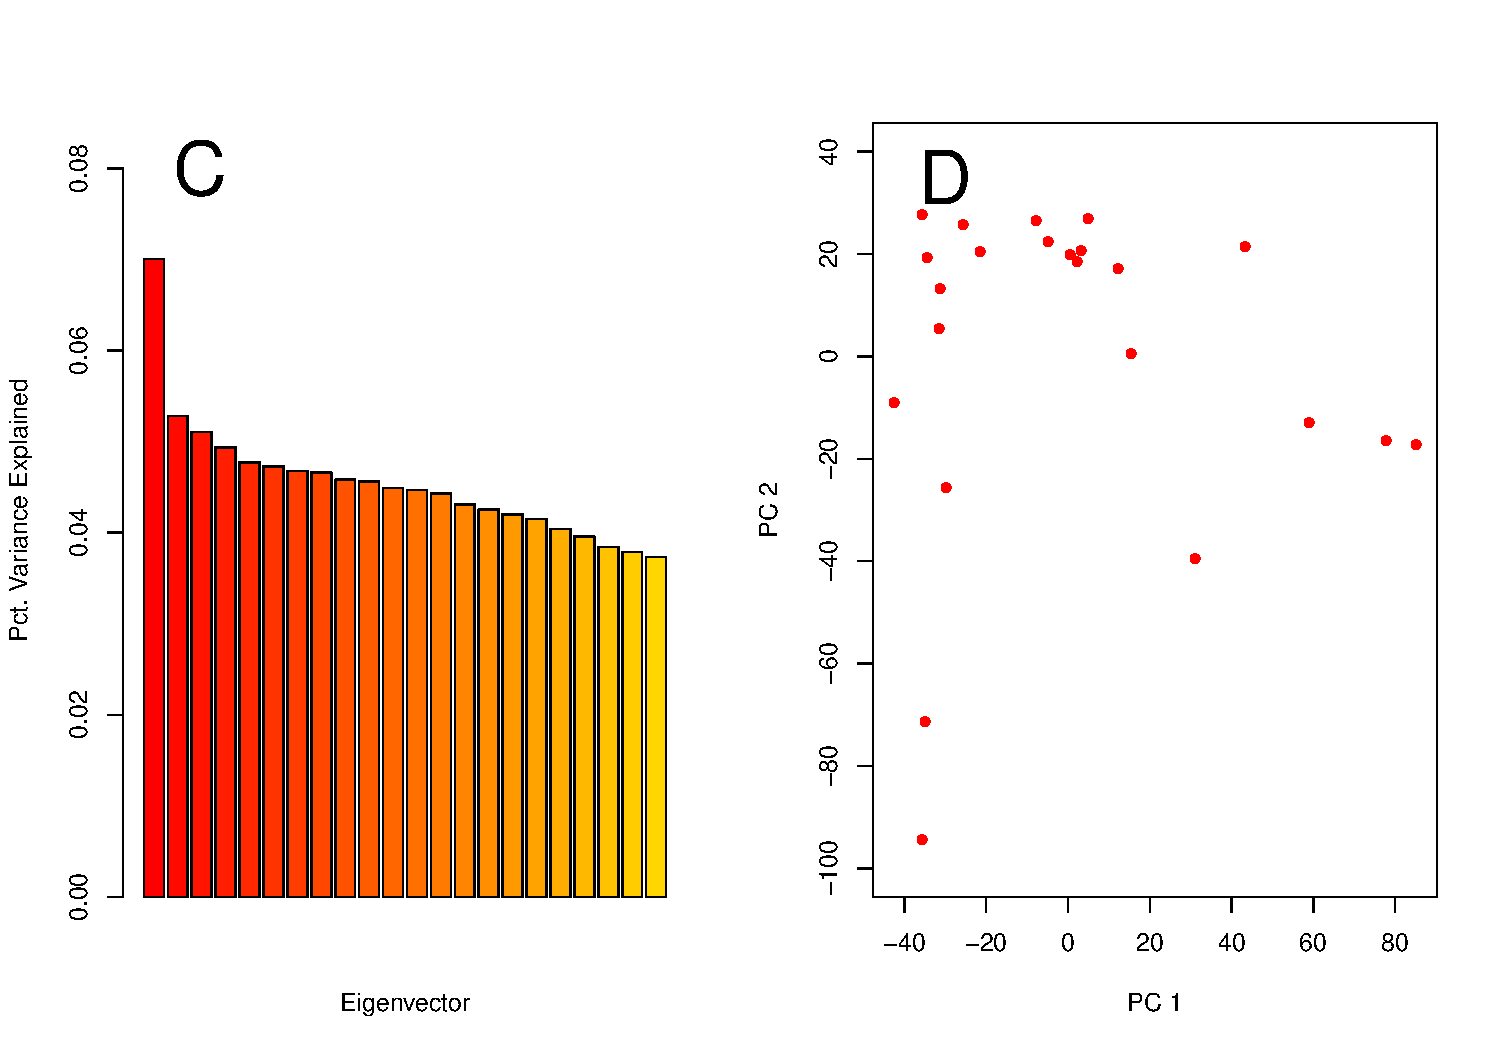
\includegraphics[width=.75\textwidth]{FigsAndFiles/bknPCA_aug.pdf}\\
  \end{center}
  \caption{Principal component analysis of teosinte and maize individuals to ensure that no close relatives were inadvertantly included in our study. Plots are based on a random sample of 10,000 SNPs. {\bf A} displays the percentage of total variance explained by each principal component for teosinte, while {\bf B} shows PC1 vs PC2 for all 13 teosinte individuals. Simlarly, {\bf C} depicts the percentage of total variance explained by each principal component for maize, and {\bf D} shows PC1 vs PC2 for all 23 maize individuals. \label{sFig:PCA}}
\end{figure}
\clearpage

\begin{table}[h]  
  \begin{center}
  \begin{tabular}{c|c}
    \bf Maize & \bf Teosinte \\ \hline \hline
    BKN009 &  TIL01 \\
    BKN010 & TIL02 \\
    BKN011 & TIL03 \\
    BKN014 & TIL04-TIP454 \\
    BKN015 & TIL07 \\
    BKN016 & TIL09 \\
    BKN017 & TIL10 \\
    BKN018 & TIL11 \\
    BKN019 & TIL12 \\
    BKN020 & TIL14-TIP498 \\
    BKN022 & TIL15 \\
    BKN023 & TIL16 \\
    BKN025 & TIL17 \\
    BKN026 & \\
    BKN027 & \\
    BKN029 & \\
    BKN030 & \\
    BKN031 & \\
    BKN032 & \\
    BKN033 & \\
    BKN034 & \\
    BKN035 & \\
    BKN040 & \\ \hline
  \end{tabular}
  \end{center}
  \caption{A list of maize and teosinte individuals included in this study. Sequencing and details were previously described by \cite{chia2012}   } \label{sTab:list}
\end{table}
\clearpage


\begin{table}
  \begin{center}
  \def\arraystretch{2}
%  \begin{center}
  \begin{tabular}{l|c|c|c}
    \bf Parameter & \bf Initial value & \bf Upper bound & \bf Lower bound\\ \hline 
    $\frac{N_b}{N_a}$ & 0.02 & $1\times10^{-7}$ & 2 \\ 
    $\frac{N_{m}}{N_a}$ & 3 & $1\times10^{-7}$ & 200 \\
    $\frac{T_b}{2N_a}$ & 0.04 & 0  & 1 \\ 
    $\frac{M_{mt}}{N_a}$ & $1\times10^{-10}$ & $1\times10^{-7}$ & 0.001 \\
    $\frac{M_{tm}}{N_a}$ & $1\times10^{-10}$ & $1\times10^{-7}$ & 0.001 \\
  \end{tabular}
  \def\arraystretch{1} % undo stretching
  \end{center}
    \caption{ Parameters, initial values, and boundaries used for model-fitting with $\delta\alpha\delta{i}$. Parameters are shown in the units utilized by $\delta\alpha\delta{i}$, although in the text simplified units are reported.    }\label{sTab:dadi}
\end{table}

